%\documentclass[handout]{beamer}
\documentclass{beamer}
\usetheme{default}
\usepackage{hyperref}
\usepackage{listings}
\title{Software Testing  Lecture 1}
\author{Justin Pearson}
\date{2020}
\setbeamertemplate{footline}[page number]
\setbeamertemplate{navigation symbols}{}
\newcommand{\recordingpause}{
\begin{frame}{Recording Pause}
  \begin{center}
    Recording Pause
  \end{center}
\end{frame}
}
\renewcommand{\recordingpause}{}
\begin{document}
\lstset{language=python}

\begin{frame}
  \maketitle
\end{frame}
\begin{frame}{Four Questions}
  \begin{itemize}
  \item Does my software work? \pause
  \item Does my software meet its specification? \pause
  \item I've changed something, does it still work? \pause
  \item How can I become a better programmer? 
  \end{itemize}
\end{frame}
\begin{frame}
  \frametitle{The Answer}
  \begin{center}
    {\Huge 
  Testing}
  \end{center}
\end{frame}
\begin{frame}{Motivation for Software Testing}
  Before we talk about what software testing is, I would like to give
  you some examples of some spectacular software failures.
  
  
\end{frame}
\begin{frame}
  \frametitle{Software Failures}

NASA's Mars lander, September 1999, crashed due to a units
    integration fault --- cost over  \$50 million.
    \begin{quote}
      The MCO MIB has determined that the root cause for the loss of
      the MCO spacecraft was the failure to use metric units in the
      coding of a ground software file, “Small Forces,” used in
      trajectory models. Specifically, thruster performance data in
      English units instead of metric units was used in the software
      application code titled SM\_FORCES (small forces). A file called
      Angular Momentum Desaturation (AMD) contained the output data
      from the SM\_FORCES software. The data in the AMD file was
      required to be in metric units per existing software interface
      documentation, and the trajectory modelers assumed the data was
      provided in metric units per the
      requirements.\footnote{\url{ftp://ftp.hq.nasa.gov/pub/pao/reports/1999/MCO_report.pdf}}
    \end{quote}  
\end{frame}
\begin{frame}{Ariane 5 explosion}
  \begin{quote}
    Flight 501, which took place on Tuesday, June 4, 1996, was the
    first, and unsuccessful, test flight of the European Space
    Agency's Ariane 5 expendable launch system. Due to an error in the
    software design (inadequate protection from integer overflow), the
    rocket veered off its flight path 37 seconds after launch and was
    destroyed by its automated self-destruct system when high
    aerodynamic forces caused the core of the vehicle to
    disintegrate. It is one of the most infamous computer bugs in
    history.
  \end{quote}
\end{frame}
\begin{frame}[fragile]
  \frametitle{Exception Handling}
\begin{lstlisting}
 try {
  ......
 } catch (ArithmeticOverflow()) {
     ... Self Destruct .... 
   } 
\end{lstlisting}
In fact, it was an integration problem. The software module was implemented for
Ariane 4 and the programers  forgot that the Ariane 5 model had a higher initial
acceleration and a different mass.  
\end{frame}
\begin{frame}{Therac-25}
  \begin{itemize}
  \item  Radiation therapy machine. At least 6 patients where given
    100 times the intended dose of radiation. 
  \item Causes are complex
    \footnote{\url{http://sunnyday.mit.edu/papers/therac.pdf}} but one
    cause identified:
    \begin{itemize}
    \item      {\bf Inadequate Software Engineering Practices} ... including:
    \end{itemize}
    \begin{quote}
     The software should be subject to extensive testing and formal
     analysis at the module and software level; system testing alone
     is not adequate.  Regression testing should be performed on all
     software changes. 
    \end{quote}
  \end{itemize}  
\end{frame}
\begin{frame}
  \frametitle{Intel's {\tt fdiv} bug}
   
Some pentiums returned
\[
\frac{4195835}{3145727} = 1.333739068902037589
\]
instead of 
\[
\frac{4195835}{3145727} = 1.333820449136241002
\]

\end{frame}
\begin{frame}
  \frametitle{Intel's {\tt fdiv} bug}
  \begin{quote}
    With a goal to boost the execution of floating-point scalar code by 3
    times and vector code by 5 times, compared to the 486DX chip, Intel
    decided to use the SRT algorithm that can generate two quotient bits per
    clock cycle, while the traditional 486 shift-and-subtract algorithm was
    generating only one quotient bit per cycle. \textcolor{red}{\em This SRT
      algorithm uses a lookup table to calculate the intermidiate quotients
      necessary for floating-point division. Intel's lookup table consists of
      1066 table entries, of which, due to a programming error, five were not
      downloaded into the programmable logic array (PLA).} When any of these
    five cells is accessed by the floating point unit (FPU), it (the FPU)
    fetches zero instead of +2, which was supposed to be contained in the
    "missing" cells. This throws off the calculation and results in a less
    precise number than the correct answer(Byte Magazine, March 1995).
  \end{quote}
\end{frame}
\begin{frame}
  \frametitle{Intel's {\tt fdiv} bug}
  \begin{itemize}
  \item Simple programming error: not getting the loop termination
    condition correct.
  \item Later we'll see that this might have been avoided with testing.
  \end{itemize}
\end{frame}
\begin{frame}
  \frametitle{Software Failures}
  \begin{itemize}
  \item These are just some of the most spectacular examples. There is
    a lot of bad software out there. Anything we can do to
    improve the quality of software is a good thing. 
  \item  Formal methods are hard to implement, but
    software testing with some discipline can become part of any
    programmer's toolbox.
  \end{itemize}
\end{frame}

\begin{frame}{The reality of Software Development}
  \begin{itemize}
  \item All code has problems.
  \item Anything that we can do to improve the quality of our code is
    important.
    
  \end{itemize}
  
\end{frame}

\recordingpause

\begin{frame}{Software Engineering and Testing}

Software Engineering tells us how to develop software. There are many
models and processes including
\begin{itemize}
\item The Waterfall Model
\item Agile Development
\item Scrum
\item Extreme Programming 
\end{itemize}
 We will not cover software engineering methodology, but it is
 important to think about how software testing fits in with your
 development process. 
\end{frame}
\begin{frame}{The V model --- Software Engineering}

\begin{center} 
 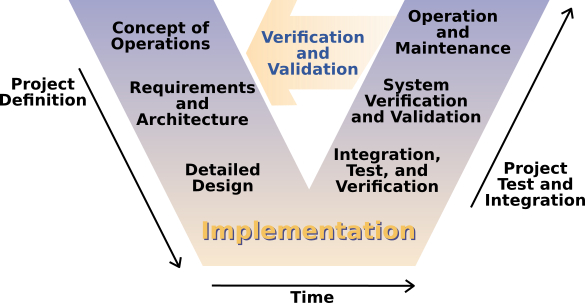
\includegraphics[height=2in,width=4in]{V_model.png}
\end{center}
Even if you don't develop software this way, it is a useful way of
thinking about software development.
\end{frame}

\begin{frame}
  \frametitle{Testing}

  There are lots of different testing activities with names inspired
  by the V model.  We cannot cover them all but they include:
  \begin{itemize}
  \item \textbf{Unit Testing}: Testing your functions/methods as you write your
    code.
  \item \textbf{Regression testing}: maintaining a possibly large set of test
    cases that have to passed when ever you make a new release.
  \item \textbf{Integration testing}: testing  if your software modules fit
    together. 
  \end{itemize}
\end{frame}
\begin{frame}
  \frametitle{Can we test?}
  
  \begin{quote}
    ``Program testing can be used to show the presence of bugs, but
    never to show their absence!'' Edsger Dijkstra.
  \end{quote}


This is true, but it is no reason to give up on testing. All software has
bugs. Anything you do to reduce the number of bugs is a good thing.
\end{frame}

\recordingpause

%\begin{frame}
%  \frametitle{Test Driven Development}
%  Later on we will look at \textit{test driven development} (TDD) which is a
%  programming discipline where you write the tests before you write
%%  the code.
%\end{frame}

\begin{frame}{What is a Test?}
  This is quite a complex question and depends on what you are
  developing.
  \begin{itemize}
  \item How do I test a GUI?
  \item How do I test a real-time system?
  \item How do I load-test a web-server?
  \item How do I test a database system?
  \end{itemize}
  How do I write code that can be tested?
  
\end{frame}
\begin{frame}
  \frametitle{What is a Test?}
In this course we will look testing functions or methods. 
  \begin{itemize}
  \item A test is simply some inputs and some expected outputs.
  \end{itemize}
  This simple description hides a lot of complexity, though.
  \begin{itemize}
  \item How do I know what my code is supposed to do, so that I can
    work out what the expected outputs are?
  \item   What exactly are the inputs and outputs of my system?
  \end{itemize}

\end{frame}

\begin{frame}
  \frametitle{Aspects of Testing}
  \begin{enumerate}
  \item Test Design
  \item Test Automation
  \item Test Execution
  \item Test Evaluation
  \end{enumerate}
It is very important that test execution should be as automated as possible. It
should be part of your {\tt Makefile}. Some systems even automatically
run tests when you check in code.
\end{frame}
\begin{frame}
  \frametitle{Test Design}
  \begin{itemize}
  \item  Writing good tests is  hard. 
  \item It requires knowledge of you  problem, and 
  \item Knowledge of common errors.
  \item Often, a test designer is a separate  position in a company.
  \item Test design helps the tester understand the system.
  \end{itemize}
\end{frame}
\begin{frame}
  \frametitle{Test Design}
  
  \begin{itemize}
  \item Adversarial view of test design: 
    \begin{quote}
       How do I break software? \pause
    \end{quote}
  \item Constructive view of test design:
    \begin{quote}
       How do I design software tests that improve the software process?
     \end{quote}
   \item Often you design tests to uncover common programming errors
     for example off by one errors.
  \end{itemize}
\end{frame}


\begin{frame}  
  \frametitle{Test Automation}
  \begin{itemize}
  \item Designing good tests is hard.
  \item If you don't make the execution of the tests an automated process, then
    people will never run them.
  \item There are many automated systems, but you can roll your own
    via scripting languages.   
  \item The xUnit framework has support in most languages for the
    automated running of tests. 
  \item It should be as simple as {\tt make tests}.
  \end{itemize}
\end{frame}
\begin{frame}
  \frametitle{Test Automation}
  \begin{itemize}
  \item There are tools for automatically testing web systems.
  \item There are tools for testing GUIs.
    \begin{itemize}
    \item If you design your software correctly you should decouple as
      much of the GUI behaviour from the rest of the program as you
      can. This will not only make your program easier to port to
      other GUIs, but also it will make it easier to test.
    \end{itemize}
  \item Don't forget to include test automation in your compilation
    process.
  \item Consider integrating automated testing into your version
    management system.  
  \end{itemize}
\end{frame}
\begin{frame}
  \frametitle{Test Execution}
You need to think of test execution as separate activity. You have to
remember to run the tests. In a large organization this might require
some planning.    
  \begin{itemize}
  \item Easy if testing is automated.
  \item Hard for some domains e.g. GUI.
  \item Very hard in distributed or real time environments.
  \end{itemize}
\end{frame}

\begin{frame}
  \frametitle{Test Evaluation}
  \begin{itemize}
  \item My software does not pass some of the tests. Is this good or
    bad?
  \item My software passes all my tests. Can I go home now? Or do I
    have to design more tests?
  \end{itemize}
\end{frame}

\recordingpause

\begin{frame}
  \frametitle{Important Terminology and Concepts}

  \begin{itemize}
  \item {\bf Validation:} The process of evaluation software at the end
    of software development to ensure compliance with intended usage.
  \item {\bf Verification:} The process of determining whether the
    products of a given phase of the software development process
    fulfill the requirements established during the previous phase
  \end{itemize}
  
\end{frame}
\begin{frame}
  \frametitle{Important Terminology and Concepts}
  \begin{itemize}
  \item  {\bf Software Fault:} A static defect in the software.
  \item {\bf Software Error:} An incorrect internal state that is the
    manifestation of some fault. 
  \item {\bf  Software Failure:} External,
    incorrect behavior with respect to the requirements or other
    description of the expected behaviour.
  \end{itemize}
Understanding the difference will help you fix faults. Write your code
so it is testable.
\end{frame}
\begin{frame}[fragile]
  \frametitle{Pop Quiz}
  How many times does this loop execute?
 \textcolor{blue}{errors}\begin{lstlisting}
  for(i=10; i<5; i++) {
     do_stuff(i);
  }
\end{lstlisting}

\end{frame}
\begin{frame}[fragile]
  \frametitle{Fault/Error/Failure Example}
\begin{lstlisting}
  int count_spaces(char* str) {
   int length, i,count;
   count = 0;
   length = strlen(str);
   for(i=1; i<length; i++)  { 
     if(str[i] == ' ') { count++; }
   }
   return(count);
  }
\end{lstlisting}
  \begin{itemize}
  \item Software Fault: {\tt i=1} should be {\tt i=0}.
  \item Software Error: some point in the program where you
    incorrectly count the number of spaces.
  \item Failure  inputs and outputs that make the fault happen. For
    example {\tt count\_spaces("H H H");} would not cause the failure
    while {\tt count\_spaces(" H");} does.
  \end{itemize}
\end{frame}
\begin{frame}
  \frametitle{Fault/Error/Failure}
  \begin{itemize}
  \item Fault/Error/Failure is an important tool for thinking about how to
    test something (not just software).
  \item I am trying to correct \textcolor{red}{faults} that cause
    \textcolor{blue}{errors} that cause \textcolor{green}{failures}.
  \item How do I design test cases that give  \textcolor{green}{failures} that
    are caused by  \textcolor{blue}{errors} that are due to
    \textcolor{red}{faults} in the code.
  \end{itemize}
\end{frame}

\begin{frame}{The RIP model}
 Reachability,  Infection and Propagation.
  \begin{itemize}
  \item Reachability: The test causes the faulty statement to be
    reached.
  \item Infection: The test case causes the faulty statement to result
    in an incorrect state.
  \item Propagation: The incorrect state propagates to incorrect output.
    \end{itemize}
  \end{frame}
  \begin{frame}{Analogy with disease}
    \begin{itemize}
    \item The symptom is only an indication of what is wrong with you.
    \item Test cases are a diagnostic tool. We can only see the
      symptoms and not inside the software. 
    \end{itemize}    
  \end{frame}




%\begin{frame}
%  \frametitle{More Testing Concepts}
%  \begin{itemize}
%  \item Sometimes you don't have all the functionality
%    implemented. Write dummy functions, {\em stubs}, that simply return
%    null values rather doing any real work. Means that you can get
%    your code going.
%  \item {\em Mock} or {\em Fake} objects (people make a distinction
%    but don't worry) implement enough of an object to get the test
%    going.
%  \end{itemize}
%In fact in test driven development you write the test, implement the
%{\em mocks} first and as you introduce more tests you add code to make the
%tests pass.
%
%\end{frame}
%\begin{frame}
%  \frametitle{Test functions}
%  \begin{itemize}
%  \item It is a matter of judgment and taste how many tests you put in
%    each function.
%  \item  You don't want individual tests  to take too much time to
%    run. This will discourage the programmer from running individual
%    test often.
%  \item Whenever you compile your code you should run the tests. 
%  \item Often IDEs implement red and green bars for tests. Green means
%    the test has passed and red means the test has failed.
%  \item Green is good. 
%  \end{itemize}
%\end{frame}
%\begin{frame}
%  \frametitle{How to use Unit Tests}
%  \begin{itemize}
%  \item When you are writing functions use test cases to see if the
%    behaviour is as expected.
%  \item Use tests as another form of documentation. Helps other
%    programmers understand your API.
%  \item When you find a bug write a test case and then correct the
%    bug. Leave the test case there just in case fixing another bug
%    reintroduces a bug.
%  \end{itemize}
%\end{frame}
%\begin{frame}[fragile]
%  \frametitle{Some things to test for}
%  \begin{itemize}
%  \item Extreme values. Empty strings, large values.
%  \item Loops executing zero, once, many times, and test the loop
%    termination condition.
%    \begin{lstlisting}
%      for(int i=0; i<M; i++) {
%        do_something(i);
%      }
%    \end{lstlisting}
% \item  Find a test case that sets {\tt M} to be 0, 1 and some larger
%   number. 
% \item Often {\tt M} will not be an input parameter. You might have to
%   work out how the input parameters affect {\tt M}
%   \begin{lstlisting}
%      void whatever(char* str) {
%         M = strlen(str); 
%         .... 
%      }
%   \end{lstlisting}
%\item  So you have to have a string  of length 0,1 and some bigger number.
%\end{itemize}
%\end{frame}
%
%\begin{frame}[fragile]
%  \frametitle{Some things to test for}
%  \begin{itemize}
%  \item Code coverage. This is a complex area, but you should not
%    really have untested code.
%    \begin{lstlisting}
%       if(X==Y) { do_something(); } 
%       else {do_something_else();}
%    \end{lstlisting}
%\item Find a test case where {\tt X} equals {\tt Y} and a test case
%  where they are different.
%  \end{itemize}
%\end{frame}
%\begin{frame}
%  \frametitle{Have a reason}
%  \begin{itemize}
%  \item You can't test code just by letting a monkey type random
%    things on the keyboard (although it sometimes helps).
%  \item Try to have a reason for every test.
%  \item Document reasons.
%  \item When you test suite gets too large you have to work out which
%    tests to delete.
%  \end{itemize}
%\end{frame}
%
\begin{frame}
  \frametitle{Suggested Reading}
  \begin{itemize}
  \item One of the testing gods is James Bach see his
    website\footnote{\url{http://www.satisfice.com/}}
  \item The book {\em Introduction to Software
      Testing}\footnote{\url{http://cs.gmu.edu/~offutt/softwaretest/}}
    by Ammann and Offutt. This is a bit theoretical. 
  \item The book {\em Test-Driven Development by Example} by Kent Beck.
    Who is one of the  fathers of unit testing, agile programming  and
    extreme programming. 
    % \item {\em Practical software testing} by Ilene Burnstein. Avaibl
    \item A classic ``The ART of software testing'' Glenford Meyers.  Online
      at the university library. 
  \end{itemize}
\end{frame}
\end{document}



%%% Local Variables:
%%% mode: latex
%%% TeX-master: t
%%% End:
